
\section{Generatore di onda quadra}
	Per la realizzazione di un generatore di onda quadra si sono impiegati il multivibratore monostabile e astabile montati precedentemente, in modo da ottenere il circuito in \figurename{ \ref{f:qadra}}.

	\begin{figure}[H]
		\begin{minipage}{0.75\textwidth}
		\centering
		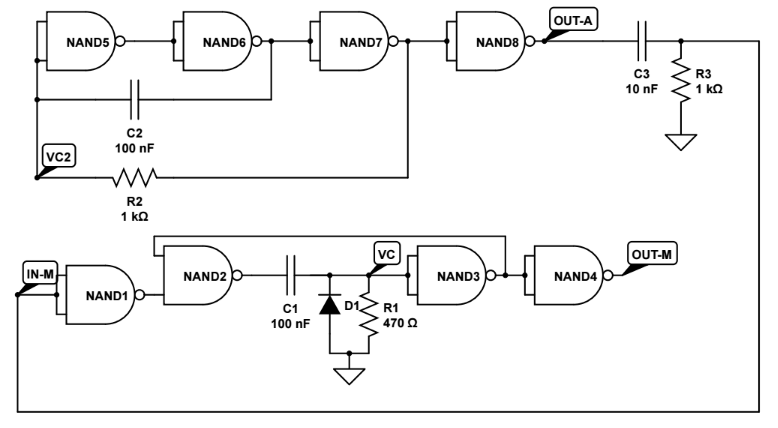
\includegraphics[scale=0.6]{qadra.png}
		\caption{schema del generatore di onde quadre}
		\label{f:qadra}
		\end{minipage}
		\begin{minipage}{0.14\textwidth}
			\begin{tabular}{l}
		$R_{3}=\SI{988 \pm 8}{\ohm}$\\
		$C_{3}=\SI{10.8 \pm 0.4 }{\nano \farad}$
			\end{tabular}
		\end{minipage}
	\end{figure}

	Si riporta in \figurename{ \ref{f:osci-qad}} l'acquisizione del segnale del multivibratore monostabile: il segnale in ingresso (ch1) e il segnale in uscita dal derivatore (ch2).

	\begin{figure}[H]
		\centering
		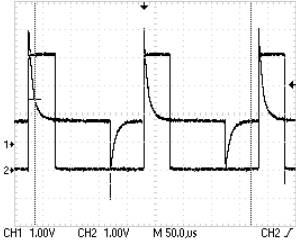
\includegraphics[scale=1.0]{deth_generator.png}
		\caption{input e output del multivibratore monostabile.}
		\label{f:osci-qad}
	\end{figure}

	Il circuito monostabile, come riscontrabile in \figurename{ \ref{f:osci-qad}},
	trasforma l'onda quadra generata dall'astabile in un impulso di breve durata temporale; sempre dalla figura in esame può essere osservato che il monostabile risulta sensibile solo al fronte di salita del segnale in ingresso.

	Come atteso in uscita al circuito monostabile si ottiene un onda quadra di periodo $T=\SI{205 \pm 1 }{\us}$ e duty cycle $D\%= 22.9 \pm 0.2$\%.

	Si è proceduto a variare separatamente i valori di $R_{1}$ e $R_{2}$, si sono ottenuti i dati in \tablename{ \ref{t:4}}.

	\begin{table}[H]
		\centering
		\begin{tabular}{cccc}
			\toprule
			$R_{1}$ [\si{\ohm}] & $R_{2}$ [\si{\kilo \ohm}] & $T$ [\si{\us}] & $\Delta T_{up}$  [\si{\us}] \\
			\midrule
			470 $\pm$ 5	&	1120 $\pm$ 10	&	234 $\pm$ 1	&	47.6 $\pm $0.2	\\
			567 $\pm$ 6	&	1120 $\pm$ 10	&	234 $\pm$ 1	&	59.2 $ \pm$ 0.4		\\
			567 $\pm$ 6	&	988 $\pm$ 9	&	205 $\pm$ 1	&	59.2 $\pm$ 0.4		\\
			\bottomrule
		\end{tabular}
		\caption{Periodo e duty cycle al variare di $R_1$ e $R_2$}
		\label{t:4}
	\end{table}

	Come possiamo osservare dai valori tabulati si osserva che la durata del semiperiodo HIGH dipende solo da $R_1$, mentre il periodo dipende solo da $R_2$.

	\paragraph{}Si è adesso proceduto a realizzare un generatore di onde quadre di $T\simeq \SI{100}{\us} $ e $D \% \simeq 30 \% $.

	Dai valori ottenuti nelle sezioni precedenti abbiamo stimato per i valori richiesti delle resistenze attese ${R_{1}}^{exp}=\SI{306(9)}{\ohm}$ e ${R_{2}}^{exp}=\SI{474 \pm 6}{\ohm}$. %R1 place holder
	% non sono riuscito a trovare il simbolo pentacolo in LaTeX, mi sembra una grave mancanza
	Si è osservato tuttavia che impiegando tali resistori si ottiene un impulso sensibilmente diverso da quello atteso, si è pertanto proceduto a variare i valori delle resistenze (per mezzo di potenziometri) sino ad ottenere i valori voluti di periodo e duty cycle.

	Al termine di tale processo sono state impiegate delle resistenze $R_{1}=$\SI{331 \pm 3}{\ohm} e $R_{2}=$\SI{464 \pm 4}{\ohm} ottenendo $T=$\SI{101 \pm 1}{\us} e $ D\%=$\SI{29.9 \pm 0.4}{\%}.

	Una causa della leggera discrepanza rispetto ai valori attesi potrebbe essere imputabile all'andamendo non esattamente lineare dei tempi con le resistenze.
